\begin{figure*}[thb]
\centering
% \setlength{\abovecaptionskip}{0pt plus 3pt minus 2pt}
% \setlength{\belowcaptionskip}{-35pt plus 3pt minus 2pt}
% \caption*{}
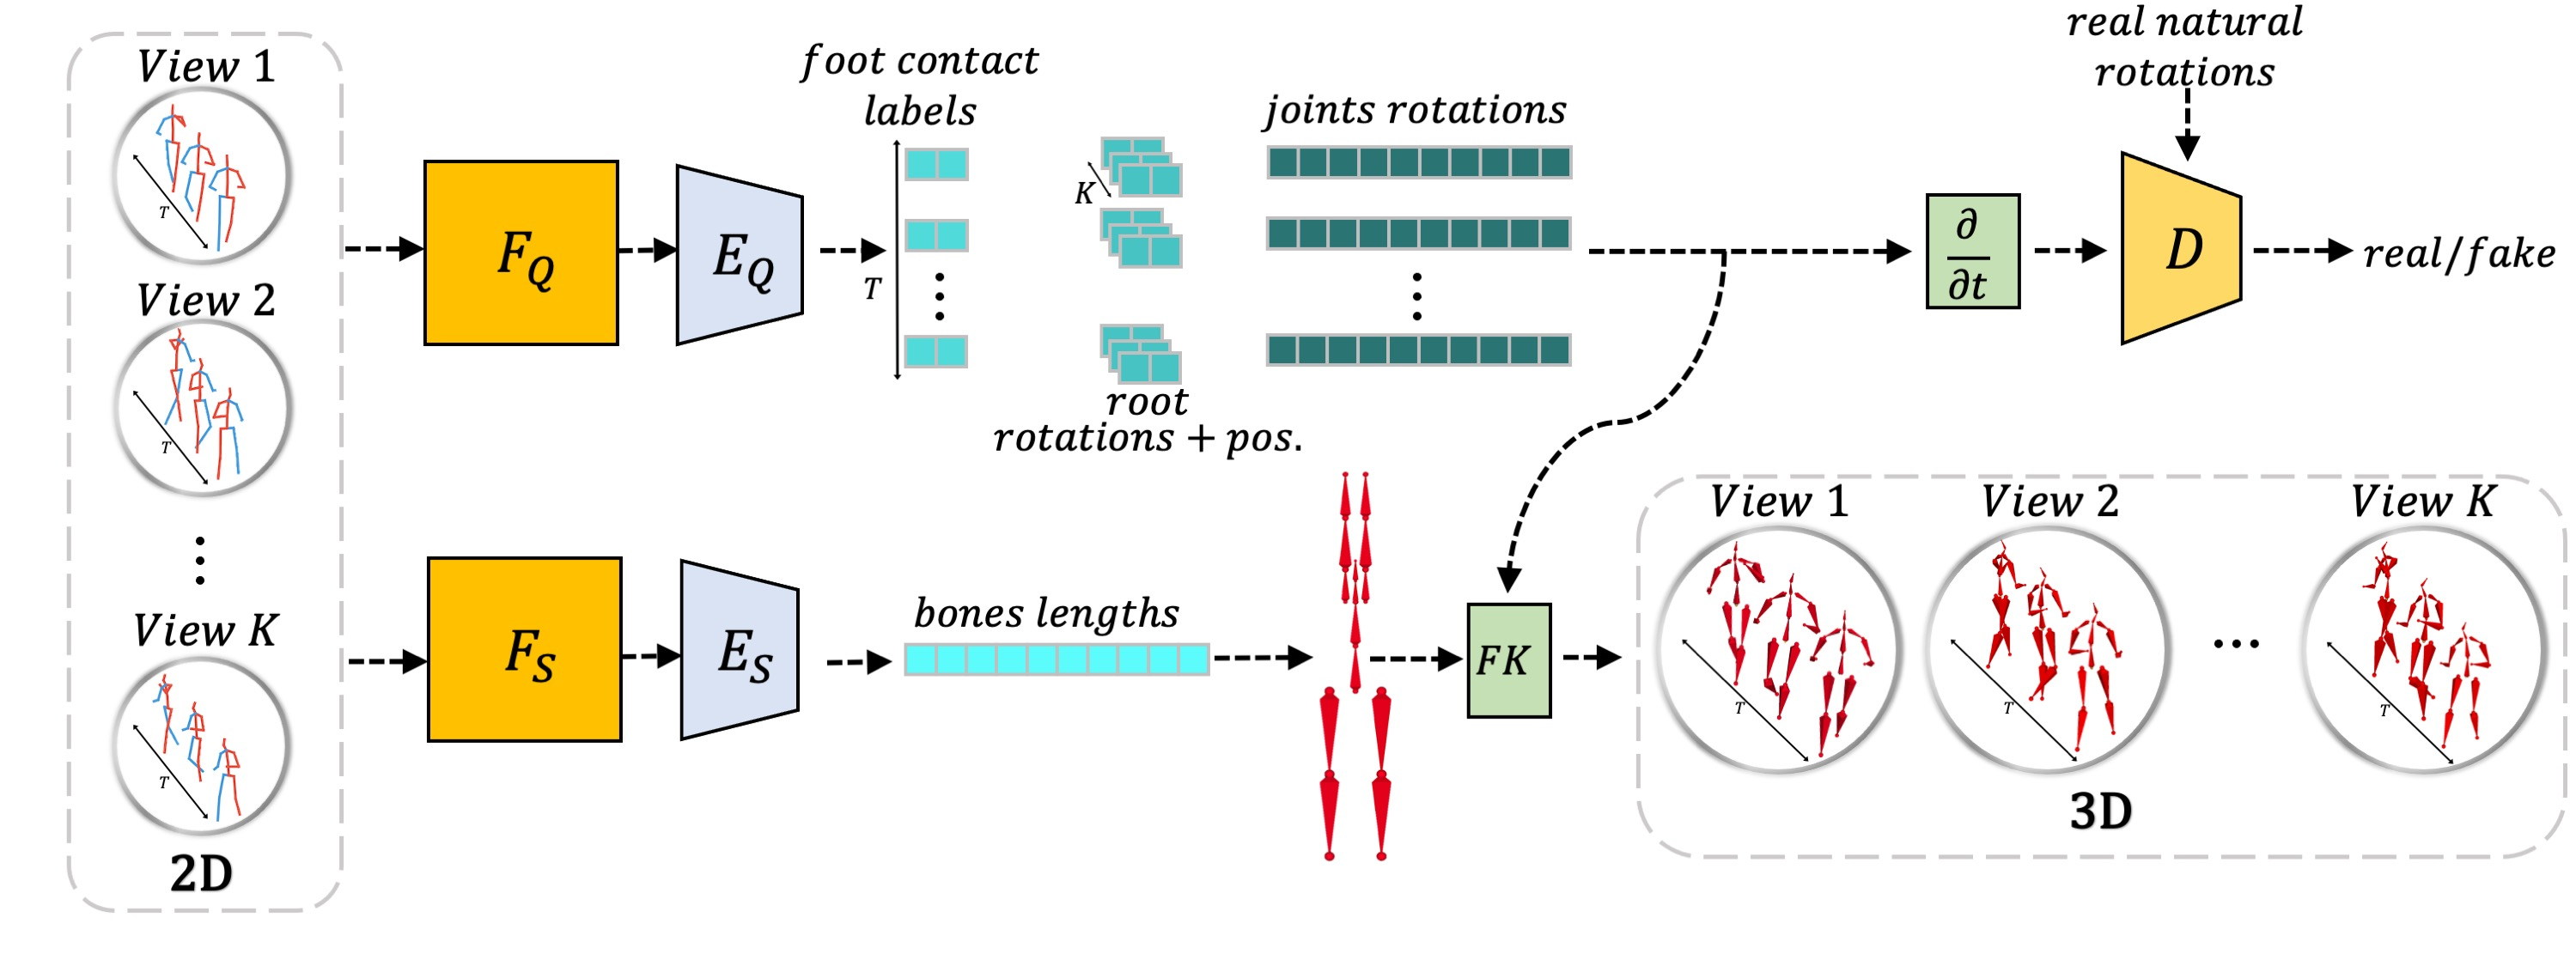
\includegraphics[width=0.9\textwidth]{./images/High_Level_Architecture.jpg}
\setlength{\abovecaptionskip}{0pt plus 3pt minus 2pt}
\setlength{\belowcaptionskip}{-15pt plus 3pt minus 2pt}
\caption{
%FLEX takes multi-view temporal sequences of 2D poses accompanied by a confidence value per joint. 
%
%Using two encoders, $E_Q$ and $E_S$, it extracts per-frame 3D joint rotations and foot contact labels, per-view and per-frame 3D root transformations, and a 3D static skeleton. 
%
%Employing a discriminator, $D$, it brings the temporal differences of rotation angles near the manifold of true rotations.
%
%Applying a forward kinematic layer, $FK$, it extracts 3D joint positions from rotations and static features, which in turn are compared to ground-truth.
%
FLEX takes multi-view temporal sequences of 2D poses and their confidence values. 
%
It uses two encoders, $E_Q$ and $E_S$, to extracts per-frame 3D rotations and foot contact labels, per-view and per-frame 3D root transformations, and one static skeleton. 
%
%
A discriminator $D$ monitors the temporal differences of rotation angles,
%
and a forward kinematic layer, $FK$, 
%extracts 3D joint locations from rotations and bone lengths,
combines encoders' outputs into 3D joint locations.
%, which in turn are compared to ground-truth.
%
\sr{These outputs depict \emph{one} human, transformed into the axis systems of $K$ cameras, to be compared with $K$ sets of  ground-truth values.}
% are identical except for their root transformation. 
% We compute $K$ outputs (rather than one) for the purpose of loss computation vs. $K$ ground-truth sets of values. 
}

\label{fig:architecture_concept}
\end{figure*}